\documentclass[12pt]{article}
\usepackage[margin=1in]{geometry}
\usepackage{graphicx}
\usepackage{booktabs}
\usepackage{amsmath}
\usepackage{amssymb}
\usepackage{float}
\usepackage{caption}
\usepackage{setspace}
\usepackage[most]{tcolorbox}
\captionsetup{font=small, labelfont=bf, skip=6pt}
\onehalfspacing
\graphicspath{{figures/}}

\newtcolorbox{explain}{%
  colback=black!3,
  colframe=black!25,
  boxrule=0.5pt,
  arc=1pt,
  left=8pt,
  right=8pt,
  top=5pt,
  bottom=5pt,
  before skip=6pt,
  after skip=12pt,
  fontupper=\normalsize
}

\title{Train, Validation, and Test Scores\\[0.2em]
\large HAR vs LSTM}
\author{Volatility forecasting project}
\date{1 October 2026}

\begin{document}
\maketitle

\noindent
HAR and LSTM scores on every Protocol~B split.
Forecasts come from the saved parquet files
(\texttt{models/baseline\_forecasts.parquet}, \texttt{models/lstm\_forecasts.parquet}).
Runner: \texttt{reports/run\_split\_compare.py}.

\section{How to read the numbers}
\begin{itemize}
  \item Final HAR and LSTM fits use train+val (Protocol~B).
    Train and val metrics are therefore in-sample.
  \item Test (2024-01-01 through 2026-09-25, \(n=999\)) is the only clean
    out-of-sample window.
  \item The LSTM needs a lookback of \(L=60\), so the first 59 train days have
    no LSTM forecast (\(n_{\mathrm{train}}=1481\)). HAR uses all 1540 train rows.
  \item RMSE and MAE are on \(\log\mathrm{RV}\). MAPE and QLIKE are on RV.
  \item In the bar charts, MAPE is drawn as a fraction (percent$/100$) so it
    shares the vertical axis with the other three scores. Table values stay in percent.
\end{itemize}
\begin{explain}
Val was used to pick the LSTM grid and early-stopping epoch. After that choice,
the network was refit on train+val. The val column for the LSTM is therefore not
a held-out tune score from the final weights; it is the final model scored on the
val dates. The val RMSE used for model selection was \(0.482\) (tune-stage fit on train only).
\end{explain}

\section{Train}
\begin{table}[H]
\centering
\begin{tabular}{lcccc}
\toprule
Model & RMSE & MAE & MAPE (\%) & QLIKE \\
\midrule
HAR & 0.436 & 0.328 & 33.0 & 0.118 \\
LSTM & \textbf{0.423} & \textbf{0.319} & \textbf{31.0} & \textbf{0.114} \\
\bottomrule
\end{tabular}
\caption{Train scores. Bold marks the lower score in each column.}
\end{table}
\begin{figure}[H]
\centering
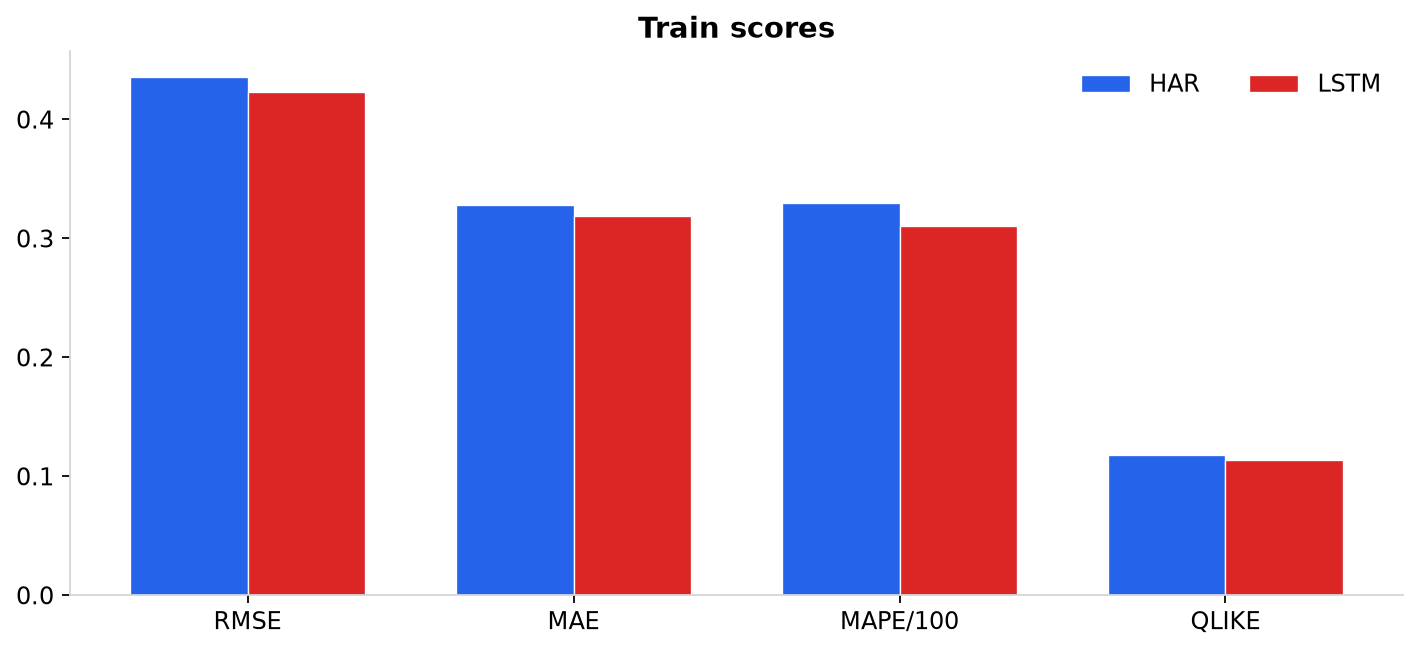
\includegraphics[width=0.95\textwidth]{split_train.png}
\caption{Train: grouped bars for HAR and LSTM on each metric.
MAPE is shown as a fraction (percent$/100$).}
\end{figure}

\section{Validation}
\begin{table}[H]
\centering
\begin{tabular}{lcccc}
\toprule
Model & RMSE & MAE & MAPE (\%) & QLIKE \\
\midrule
HAR & 0.485 & 0.372 & 41.6 & 0.125 \\
LSTM & \textbf{0.478} & \textbf{0.365} & \textbf{40.0} & \textbf{0.122} \\
\bottomrule
\end{tabular}
\caption{Validation scores. Bold marks the lower score in each column.}
\end{table}
\begin{figure}[H]
\centering
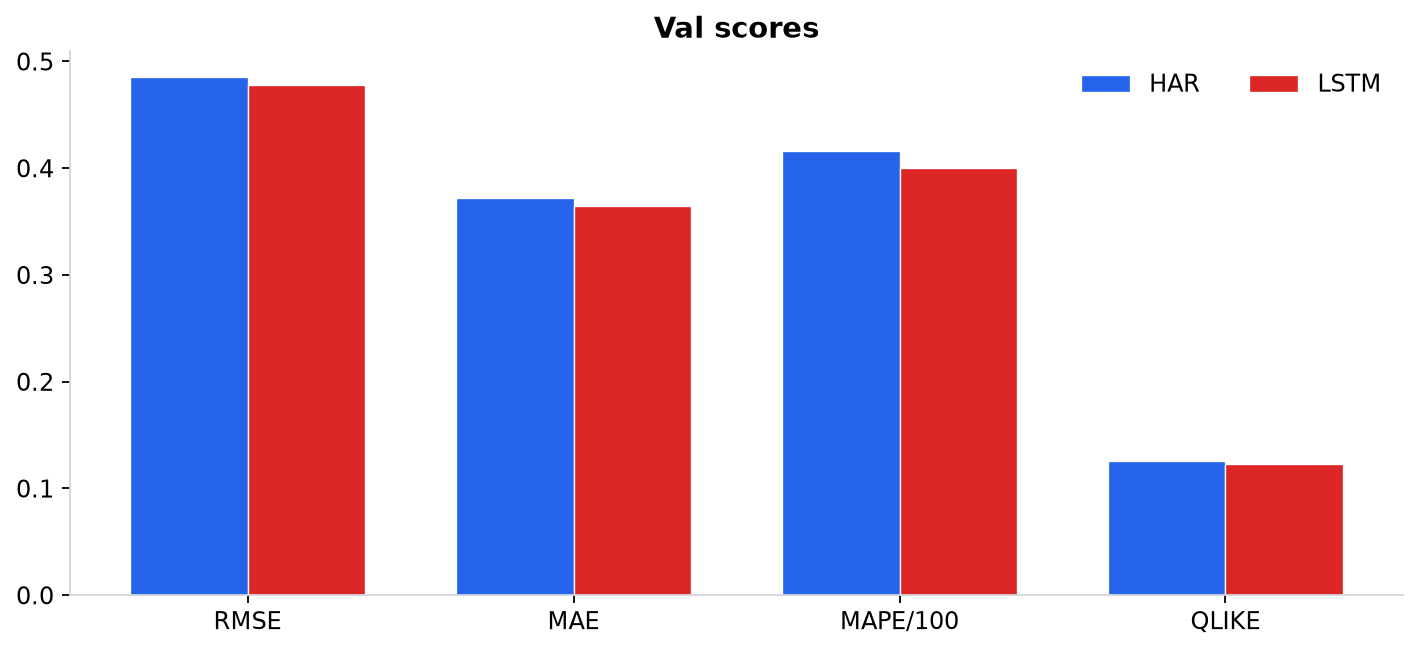
\includegraphics[width=0.95\textwidth]{split_val.png}
\caption{Validation: grouped bars for HAR and LSTM on each metric.
MAPE is shown as a fraction (percent$/100$).}
\end{figure}

\section{Test}
\begin{table}[H]
\centering
\begin{tabular}{lcccc}
\toprule
Model & RMSE & MAE & MAPE (\%) & QLIKE \\
\midrule
HAR & 0.458 & \textbf{0.354} & 40.7 & \textbf{0.101} \\
LSTM & \textbf{0.454} & 0.354 & \textbf{39.2} & 0.103 \\
\bottomrule
\end{tabular}
\caption{Test scores. Bold marks the lower score in each column.
On MAE, HAR is \(0.3537\) and the LSTM is \(0.3541\).}
\end{table}
\begin{figure}[H]
\centering
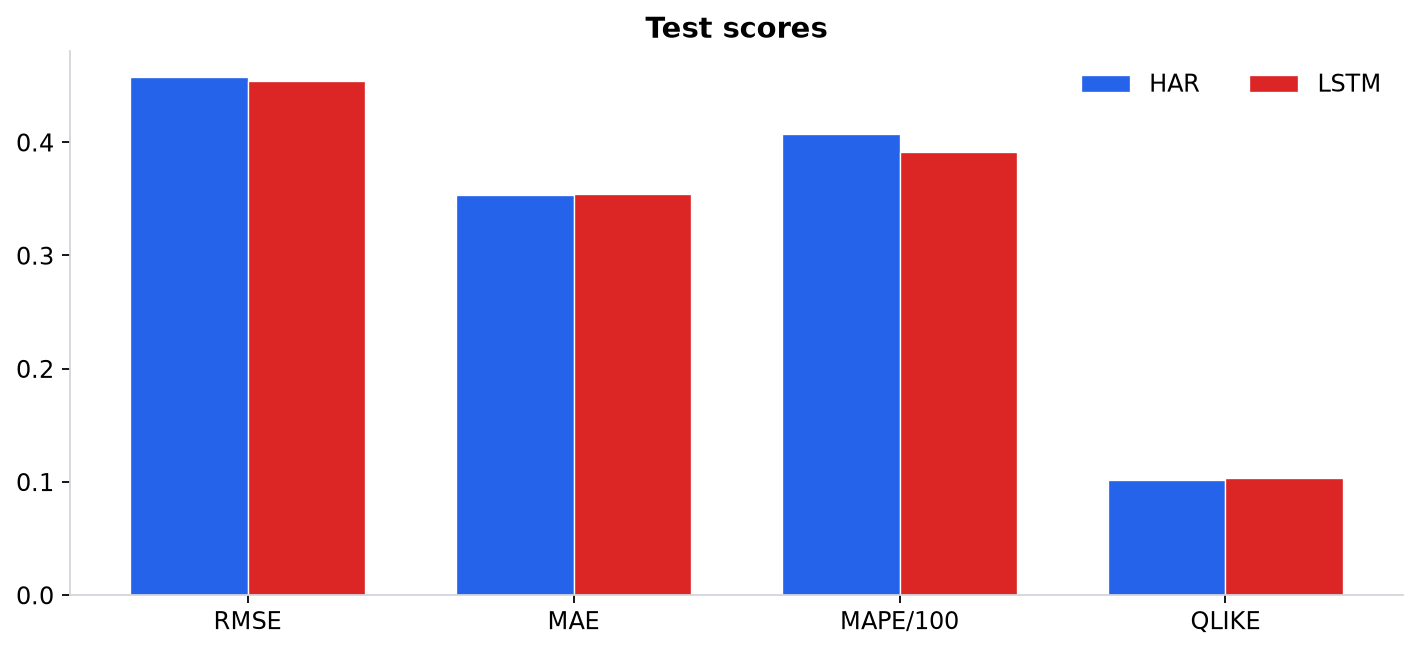
\includegraphics[width=0.95\textwidth]{split_test.png}
\caption{Test: grouped bars for HAR and LSTM on each metric.
MAPE is shown as a fraction (percent$/100$).}
\end{figure}

\section{Takeaway}
\begin{explain}
On train and val, the LSTM is lower on every score. Those columns are in-sample
after the train+val refit, so they are not a fair bake-off. On test, the LSTM is
lower on RMSE and MAPE, HAR is lower on QLIKE, and MAE is essentially tied.
\end{explain}

\end{document}
